\section{Zielsetzung}
Im Versuch wird Licht als elektromagnetische Welle am Spalt gebeugt und anschließend das
hinter dem Spalt entstehende Interferenzmuster untersucht. Es werden Spaltbreiten
zweier Einzelspalten und die Spaltbreite eines Doppelspalts untersucht.

\section{Theorie}
Unter Beugung wird verstanden, dass Wellen an einem Hindernis abgelenkt werden und
sich auf Grund dessen neue Wellenfronten nach dem Huygen'schen Prinzip bilden.
Licht wird immer dann gebeugt, wenn es durch Öffnungen in Schirmen scheint, deren Breite
etwas schmaler als der Strahldurchmesser des Lichtes ist.
Es können dabei zwei Arten der Beugung beobachtet werden: Die Fresnel'sche und die
Frauenhofer'sche Beugung.Beide Arten der Beugung sind schematisch in Abbildung \ref{abb1}
zu sehen. Bei der Fresnel'schen Beugung ist der Abstand zwischen Lichtquelle und Öffnung
und zwischen Öffnung und Bild endlich. Bei der Frauenhofer'schen Beugung hingegen sind diese
Abstände unendlich groß. Dadurch sind die miteinander inteferierenden Lichtstrahlen parallel
und werden im Gegensatz zur Fresnel'schen Beugung alle unter dem selben Winkel gebeugt.
Da es mathematisch deutlich einfacher ist, wenn alle Lichtstrahlen unter dem selben Winkel
gebeugt werden, wird im Versuch lediglich die Frauenhofer'sche Beugung betrachtet.
\FloatBarrier

\begin{figure}
  \centering
  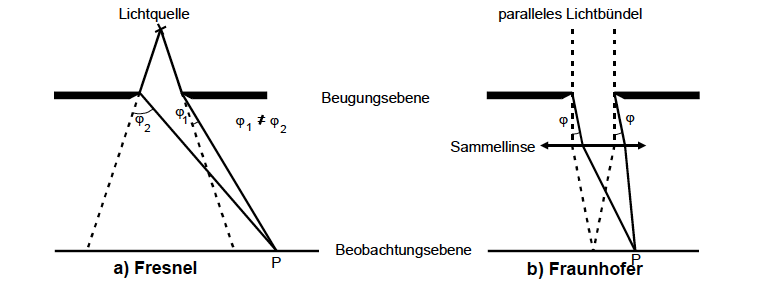
\includegraphics[scale=0.5]{Strahlen.PNG}
  \caption{Fresnel'sche und Frauenhofer'sche Beugung im Vergleich mit der geometrischen
  Optik(gestrichelte Linien). \cite{Q1}}
  \label{abb1}
\end{figure}

\FloatBarrier
Die Frauenhofer'sche Beugung ist lediglich die mathematische Formulierung des Huygen'schen Prinzips,
welches besagt, dass von jedem Punkt einer Wellenfront eine Elementarwelle ausgeht, die eine
Kugelwelle ist. Diese Elementarwellen interferieren miteinander und deren Einhüllende ist die neue
Wellenfront. Der Schwingungszustand am Beobachtungspunkt ergibt sich, wenn alle an diesem Punkt
gleichzeitig eintreffenden Elementarwellen aufsummiert werden. Am Einzelspalt muss demnach über
alle Strahlen summiert werden muss, die unter dem selben Winkel $\Phi$ gebeugt werden.
Dabei beträgt die Feldstärke, der in z-Richtung einfallenden ebenen Welle:
\begin{align*}
  A(z,t) = A_0 \symup{exp}\left(i\left(\omega~t - \frac{2\pi~z}{\lambda}\right)\right)
\end{align*}

In Abbildung \ref{abb2} wird deutlich, dass der Phasenunterschied der einzelnen eintreffenden
Lichtstrahlen
\FloatBarrier
\begin{align*}
  \delta = \frac{2~\pi~s}{\lambda} = \frac{2~\pi~x~\symup{sin}(\varphi)}{\lambda}
\end{align*}
\FloatBarrier
beträgt.
\begin{figure}
  \centering
  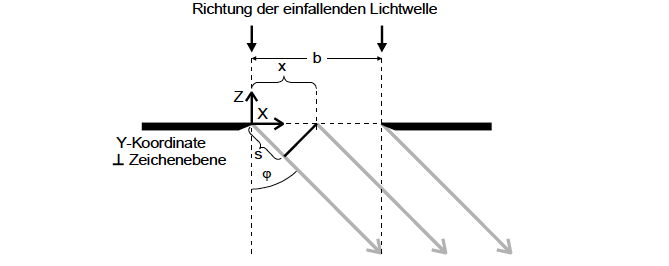
\includegraphics[scale=0.7]{phi.PNG}
  \caption{Phasenbeziehung zweier eintreffender Lichtstrahlen bei der Frauenhofer'schen Beugung
  am Spalt. \cite{Q1}}
  \label{abb2}
\end{figure}
\FloatBarrier
Um die Amplitude in $\varphi$ Richtung zu bekommen, wird über die gesamte Spaltbreite $b$ imtegriert,
da die einfallenden Lichtsrahlen infenitessimal klein sind:

\begin{align*}
  B(z, t, \varphi) = A_0 \symup{exp}\left( i \left( \omega~t - \frac{2\pi~z}{\lambda} \right) \right) \symup{exp} \left( \frac{\pi~i~b \symup{sin}(\varphi)}{\lambda}\right) \frac{\lambda}{\pi~\symup{sin}(\varphi)}\symup{sin} \left(\frac{\pi~b~\symup{sin}(\varphi)}{\lambda} \right)
\end{align*}

\newpage
Dabei werden nur reellwertige Faktoren betrachtet. Eine Amplitudenfunktion ist in Abbildung \ref{abb3} zu sehen.
Aufgrund der sehr hohen Amplitude des einfallnden Lichts wird die zeitlich gemittelte Intensität des Lichts
gemessen, welche sich mit Hilfe folgender Formel berechnen lässt:
\FloatBarrier
\begin{align*}
  I(\varphi) \propto B(\varphi)^2 = A_0^2~b^2 \left(\frac{\lambda}{\pi~\symup{sin}(\varphi)}\right)^2 \symup{sin}^2\left(\frac{\pi~b~\symup{sin}(\varphi)}{\lambda}\right)
\end{align*}
\FloatBarrier
\begin{figure}
  \centering
  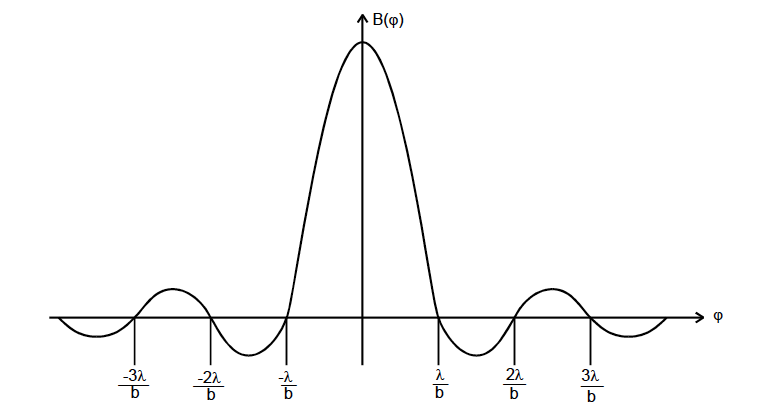
\includegraphics[scale=0.4]{amp.PNG}
  \caption{Amplitudenverteilung bei Frauenhofer'scher Beugung am Einzelspalt. \cite{Q1}}
  \label{abb3}
\end{figure}

\noindent Die Intensitätsverteilung bei der Beugung am Doppelspalt lässt sich als Überlagerung
zweier Einzelspalte betrachten, was in Abbildung \ref{abb4} gut zu sehen ist.
Folglich ergibt sich für die Intensität am Beobachtungspunkt:
\begin{align*}
  I(\varphi) \propto B(\varphi)^2 = 4 \symup{cos}^2\left(\frac{\pi~s~\symup{sin}(\varphi)}{\lambda}\right) \left(\frac{\lambda}{\pi~\symup{sin}(\varphi)}\right)^2 \symup{sin}^2\left(\frac{\pi~b~\symup{sin}(\varphi)}{\lambda}\right) .
\end{align*}
\FloatBarrier
\begin{figure}
  \centering
  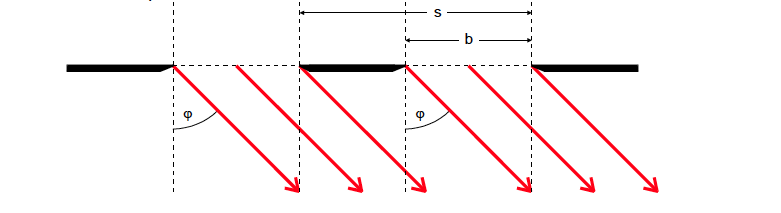
\includegraphics[scale=0.5]{ds.PNG}
  \caption{Schematische Darstellung der Beugung am Doppelspalt. \cite{Q1}}
  \label{abb4}
\end{figure}

\section{Durchführung}
Der versuchsaufbau ist in Abbildung \ref{abb5} gut zu sehen. Er besteht aus einem Helium-Neon-Laser,
der eine möglichst ebene Lichtwelle emittiert. Um den, bei der Frauenhofer'schen Beugung geforderten,
unendlichen Abstand zwischen Spalt und Detektor zu nähern, muss dieser Abstand $L$ mindestens einen Meter
betragen. Der Detektor muss dabei senkrecht zum Lichtstrahl zu verschieben sein.
\begin{figure}
  \centering
  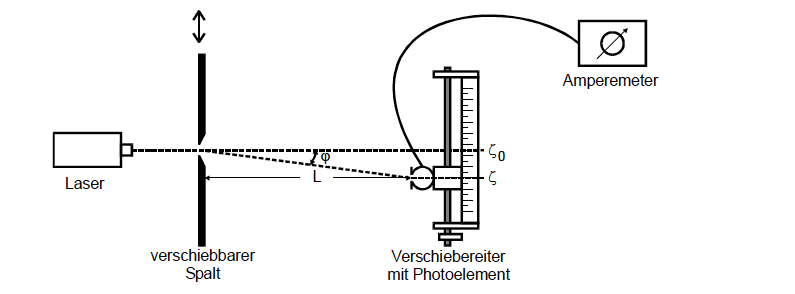
\includegraphics[scale=0.7]{aufbau.PNG}
  \caption{Versuchsaufbau \cite{Q1}}
  \label{abb5}
\end{figure}
Da die Messung nicht bei absoluter Dunkelheit durchgeführt werden kann, ist zu beachten,
dass vor der Durchführung des Experiments der Dunkelstrom einmal gemessen wird und von
den Messwerten abgezogen werden muss.
Um die Längenskala am Detektor in den Beugungswinkel $\phi$ umzurechnen, wird folgende
Formel verwendet:
\begin{align*}
  \phi \approx tan(\Phi) = \frac{\zeta - \zeta_0}{L}.
\end{align*}
$\zeta_0$ beschreibt dabei die Detektorstellung für die Richtung des ungebeugten Strahls.
Um die Beugungsmuster zu analysieren, werden zunächst die Maxima grob bestimmt, um zu
ermittlen, in welchen Bereichen mehr Messwerte aufgenommen werden. anschließend werden
die Beugunsgmuster zweier Einzelspalte und eines Doppelspalts untersucht, indem die
Intensitäten der einfallenden gebeugten und interferierenden Lichtsrahlen in verschiedenen
Detektorstellungen gemessen werden. Die Lichtintensität und die jeweilig dazugehörige
Detektorstellung werden notiert.

\section{Auswertung}

Der Abstand L zwischen dem optischen Element und der Messsonde und die Wellenlänge $\lambda$ beträgt

\begin{align*}
  L &= \SI{1,12}{\meter} \\
  \lambda &= \SI{633}{\nano\meter} .
\end{align*}

Da der Raum nicht ganz abgedunkelt werden kann, wird der Dunkelstrom
$I_{\symup{du}}$ von der Intensität bzw. dem Strom  $I$ abgezogen. Außerdem wird eine Verschiebung der Nulllinie um den Wert $\delta d$ durchgeführt.

\begin{align*}
  I_{\symup{du}} &= \SI{8}{\nano\ampere} \\
  \Delta d &= \SI{24,75}{\milli\meter} \, .
\end{align*}

\subsection{Erster Einzelspalt}

Die Werte zur Messung des ersten Einzelspaltes sind in Tabelle \ref{tab:1} aufgelistet. Die nichtlineare Regression (siehe Abbildung \ref{plot:1}) der Form

\begin{equation}
  I(\varphi) = A_0^2 b^2 \left( \frac{\lambda}{\pi b \sin(\varphi)} \right) \cdot \sin^2 \left( \frac{\pi b \sin(\varphi)}{\lambda} \right)
\end{equation}

wobei $b$ die Spaltbreite und $A_0$ eine Proportionalitätskonstante ist, ergibt

\begin{equation*}
  b = \SI{14,97(7)e-5}{\meter} .
\end{equation*}

\begin{figure}
  \centering
  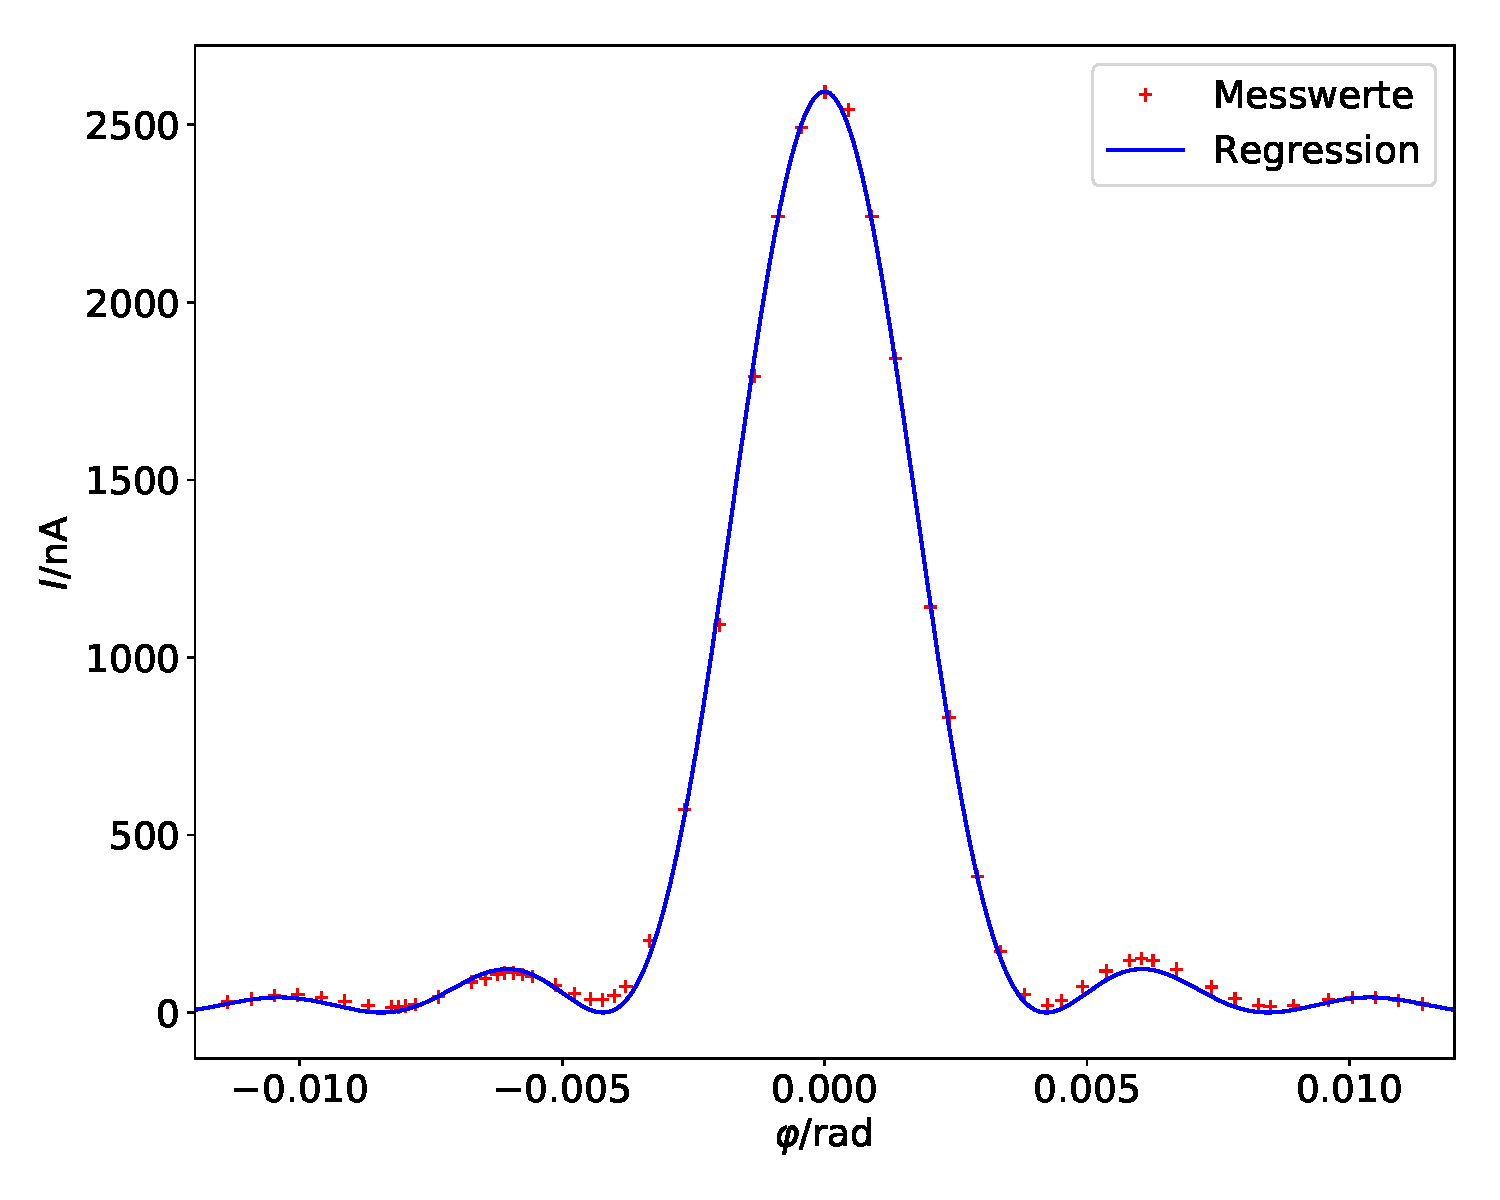
\includegraphics[scale = 0.5]{einzel.pdf}
  \caption{Messwerte und Regression der Messung am ersten Spalt.}
  \label{plot:1}
\end{figure}

\begin{table}
  \centering
  \caption{Messwerte erster Einzelspalt.}
  \label{tab:1}
  \begin{tabular}{c c || c c }
    \toprule
    $d$ / \si{\milli\meter} & $I$ / \si{\micro\ampere} & $d$ / \si{\milli\meter} & $I$ / \si{\micro\ampere} \\
    \midrule
    12.00 & 0.038 & 23.75 & 2.25 \\
    12.50 & 0.046 & 24.25 & 2.50 \\
    13.00 & 0.056 & 24.75 & 2.60 \\
    13.50 & 0.058 & 25.25 & 2.55 \\
    14.00 & 0.051 & 25.75 & 2.25 \\
    14.50 & 0.040 & 26.25 & 1.85 \\
    15.00 & 0.027 & 27.00 & 1.15 \\
    15.50 & 0.023 & 27.40 & 0.84 \\
    15.65 & 0.024 & 28.00 & 0.39 \\
    15.80 & 0.026 & 28.50 & 0.18 \\
    16.00 & 0.031 & 29.00 & 0.058 \\
    16.50 & 0.052 & 29.50 & 0.029 \\
    17.20 & 0.094 & 29.80 & 0.042 \\
    17.50 & 0.103 & 30.25 & 0.082 \\
    17.75 & 0.115 & 30.75 & 0.125 \\
    17.90 & 0.120 & 31.25 & 0.155 \\
    18.10 & 0.120 & 31.50 & 0.160 \\
    18.30 & 0.115 & 31.75 & 0.155 \\
    18.50 & 0.110 & 32.25 & 0.130 \\
    19.00 & 0.085 & 33.00 & 0.080 \\
    19.75 & 0.046 & 33.50 & 0.048 \\
    19.40 & 0.062 & 34.00 & 0.029 \\
    20.00 & 0.044 & 34.25 & 0.025 \\
    20.25 & 0.055 & 34.75 & 0.028 \\
    20.50 & 0.082 & 35.50 & 0.044 \\
    21.00 & 0.21 & 36.00 & 0.051 \\
    21.75 & 0.58 & 36.50 & 0.050 \\
    22.50 & 1.10 & 37.00 & 0.042 \\
    23.25 & 1.80 & 37.50 & 0.032 \\
    \bottomrule
    \end{tabular}
\end{table}
\newpage

\subsection{Zweiter Einzelspalt}

Die Werte zur Messung des zweiten Einzelspaltes sind in Tabelle \ref{tab:2} aufgelistet. Die nichtlineare Regression (siehe Abbildung \ref{plot:2}) der Form

\begin{equation}
  I(\varphi) = A_0^2 b^2 \left( \frac{\lambda}{\pi b \sin(\varphi)} \right) \cdot \sin^2 \left( \frac{\pi b \sin(\varphi)}{\lambda} \right)
\end{equation}

ergibt für die Spaltbreite $b$

\begin{equation*}
  b = \SI{7,87(8)e-5}{\meter} .
\end{equation*}

\begin{figure}
  \centering
  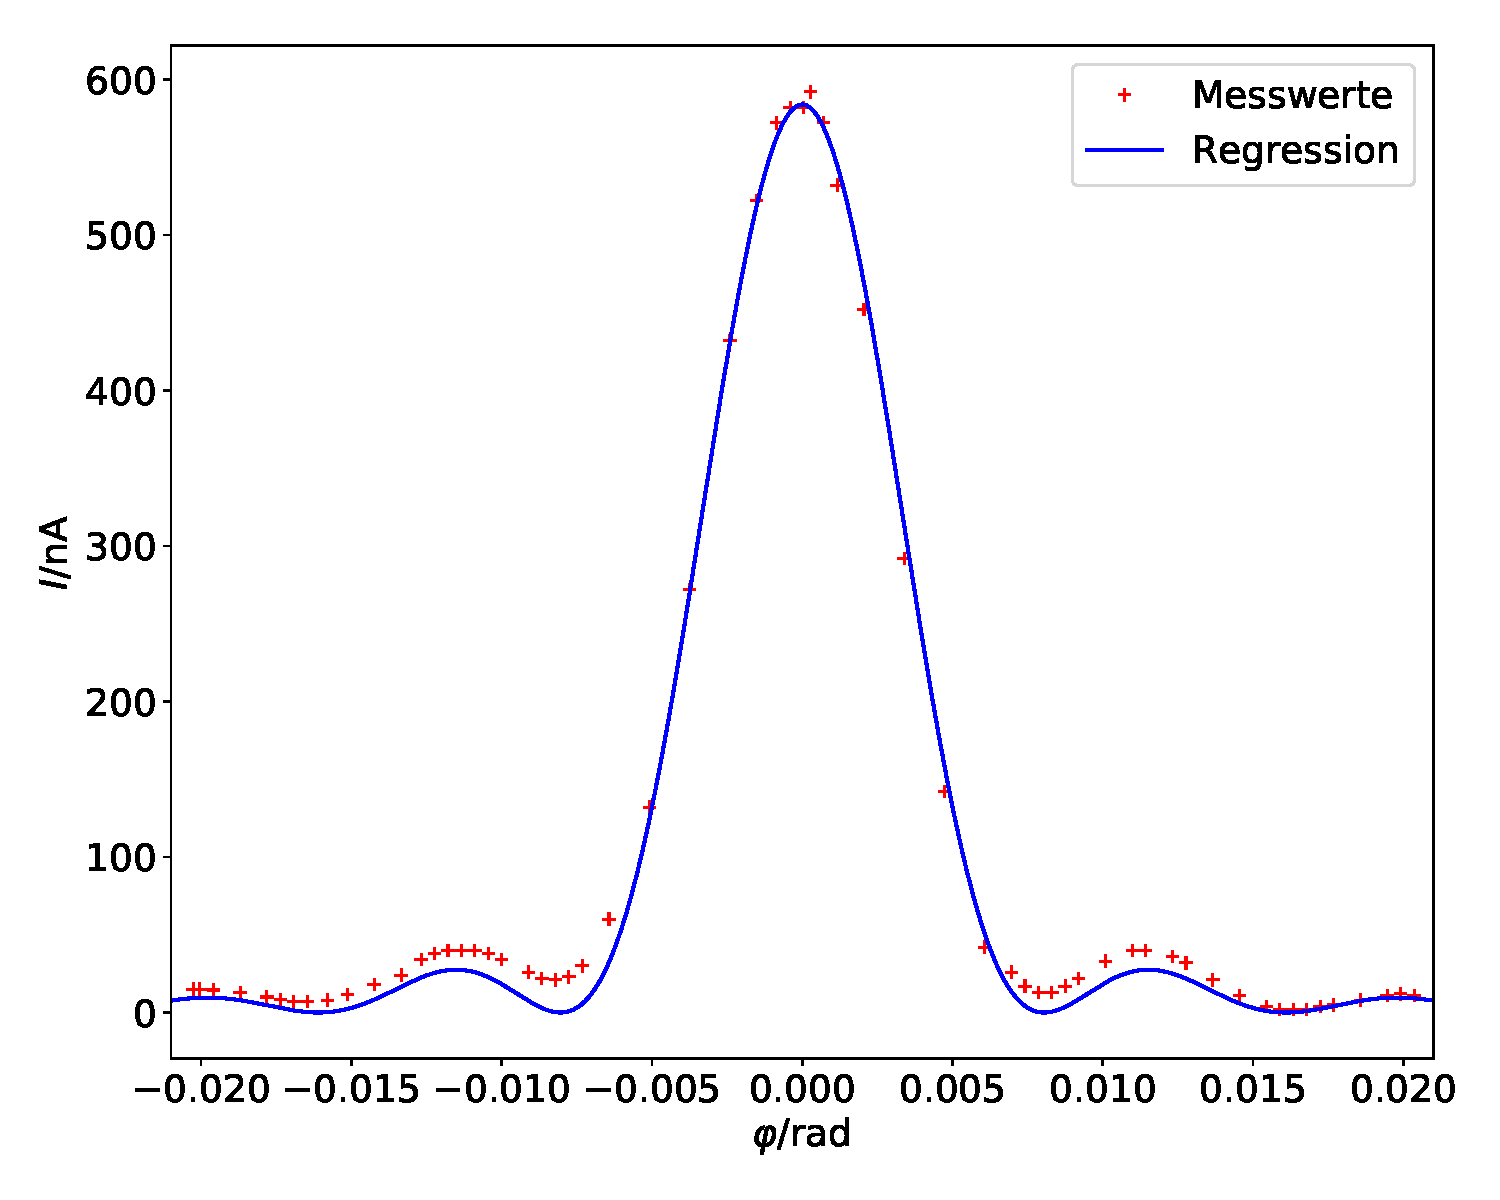
\includegraphics[scale = 0.5]{einzel2.pdf}
  \caption{Messwerte und Regression der Messung am zweiten Spalt.}
  \label{plot:2}
\end{figure}

\begin{table}
  \centering
  \caption{Messwerte zweiter Einzelspalt.}
  \label{tab:2}
  \begin{tabular}{c c || c c}
    \toprule
    $d$ / \si{\milli\meter} & $I$ / \si{\micro\ampere} & $d$ / \si{\milli\meter} & $I$ / \si{\micro\ampere} \\
    \midrule
    2.00 & 0.023  & 25.00 & 0.60  \\
    2.25 & 0.023  & 25.50 & 0.58  \\
    2.75 & 0.0225 & 26.00 & 0.54  \\
    3.75 & 0.0210 & 27.00 & 0.46  \\
    4.75 & 0.0180 & 28.50 & 0.30  \\
    5.25 & 0.0165 & 30.00 & 0.15  \\
    5.75 & 0.0150 & 31.50 & 0.05  \\
    6.25 & 0.0150 & 32.50 & 0.034 \\
    7.00 & 0.0160 & 33.00 & 0.025 \\
    7.75 & 0.0195 & 33.50 & 0.021 \\
    8.75 & 0.0260 & 34.00 & 0.021 \\
    9.75 & 0.032  & 34.50 & 0.025 \\
    10.50 & 0.042 & 35.00 & 0.030 \\
    11.00 & 0.046 & 36.00 & 0.041 \\
    11.50 & 0.048 & 37.00 & 0.048 \\
    12.00 & 0.048 & 37.50 & 0.048 \\
    12.50 & 0.048 & 38.50 & 0.044 \\
    13.00 & 0.046 & 39.00 & 0.040 \\
    13.50 & 0.042 & 40.00 & 0.029 \\
    14.50 & 0.034 & 41.00 & 0.019 \\
    15.00 & 0.030 & 42.00 & 0.012 \\
    15.50 & 0.029 & 42.50 & 0.010 \\
    16.00 & 0.031 & 43.00 & 0.010 \\
    17.50 & 0.068 & 43.50 & 0.010 \\
    17.50 & 0.068 & 44.00 & 0.012 \\
    19.00 & 0.14 & 44.50 & 0.013 \\
    20.50 & 0.28 & 45.50 & 0.016 \\
    22.00 & 0.44 & 46.50 & 0.019 \\
    23.00 & 0.53 & 47.00 & 0.020 \\
    23.75 & 0.58 & 47.50 & 0.019 \\
    24.25 & 0.59 & 48.50 & 0.016 \\
    24.75 & 0.59 &  &  \\
    \bottomrule
  \end{tabular}
\end{table}

\newpage

\subsection{Doppelspalt}

Zur Messung der Spaltbreite $b$ und des Abstandes $s$ der beiden Spalten wird eine Regression der Form

\begin{equation}
  I(\varphi) = A_0^2 \cos^2\left( \frac{\pi s \sin (\varphi)}{\lambda} \right) \cdot \left( \frac{\lambda}{\pi b \sin(\varphi)} \right)^2 \cdot \sin^2 \left( \frac{\pi b \sin(\varphi)}{\lambda} \right)
\end{equation}

zu den Messwerten aus Tabelle \ref{tab:3} durchgeführt, wobei $A_0$ erneut eine Proportionalitätskonstante ist. Diese Regression liefert die Werte

\begin{align*}
  s &= \SI{47,2(5)e-5}{\meter} \\
  b &= \SI{15,7(6)e-5}{\meter} \, .
\end{align*}

Die Messwerte und die Regression sind in Abbildung \ref{Abb:3} dargestellt.

\begin{table}
  \centering
  \caption{Messwerte Doppelspalt.}
  \label{tab:3}
  \begin{tabular}{c c || c c || c c}
    \toprule
    $d$ / \si{\milli\meter} & $I$ / \si{\micro\ampere} & $d$ / \si{\milli\meter} & $I$ / \si{\micro\ampere} & $d$ / \si{\milli\meter} & $I$ / \si{\micro\ampere} \\
    \midrule
    11.40 & 0.015 & 23.20 & 3.6 & 30.00 & 0.105 \\
    11.80 & 0.018 & 23.40 & 4.3 & 30.20 & 0.175 \\
    12.20 & 0.020 & 23.44 & 4.4 & 30.40 & 0.22 \\
    12.60 & 0.022 & 23.60 & 4.0 & 30.60 & 0.25 \\
    13.00 & 0.052 & 23.80 & 3.0 & 30.70 & 0.25 \\
    13.40 & 0.083 & 24.00 & 2.0 & 30.80 & 0.23 \\
    13.80 & 0.062 & 24.06 & 1.9 & 31.00 & 0.195 \\
    14.20 & 0.040 & 24.20 & 2.1 & 31.20 & 0.145 \\
    14.60 & 0.056 & 24.40 & 3.2 & 31.40 & 0.130 \\
    14.80 & 0.060 & 24.60 & 5.1 & 31.60 & 0.175 \\
    15.00 & 0.056 & 24.80 & 6.2 & 31.80 & 0.230 \\
    15.40 & 0.033 & 24.88 & 6.3 & 32.00 & 0.25 \\
    15.80 & 0.020 & 25.00 & 5.8 & 32.20 & 0.21 \\
    16.00 & 0.023 & 25.20 & 4.2 & 32.40 & 0.15 \\
    16.40 & 0.034 & 25.40 & 2.6 & 32.60 & 0.094 \\
    16.80 & 0.040 & 25.60 & 1.9 & 32.80 & 0.051 \\
    17.00 & 0.062 & 25.80 & 2.4 & 33.00 & 0.035 \\
    17.20 & 0.105 & 26.00 & 3.6 & 33.20 & 0.032 \\
    17.60 & 0.22 & 26.20 & 4.3 & 33.40 & 0.020 \\
    17.80 & 0.21 & 26.28 & 4.4 & 33.60 & 0.024 \\
    18.00 & 0.16 & 26.40 & 4.1 & 33.80 & 0.019 \\
    18.20 & 0.13 & 26.60 & 3.0 & 33.92 & 0.018 \\
    18.40 & 0.11 & 26.80 & 1.7 & 34.20 & 0.028 \\
    18.60 & 0.13 & 27.00 & 0.8 & 34.40 & 0.044 \\
    18.80 & 0.17 & 27.20 & 0.7 & 34.60 & 0.064 \\
    19.00 & 0.21 & 27.40 & 0.9 & 34.80 & 0.082 \\
    19.40 & 0.16 & 27.60 & 1.1 & 35.00 & 0.086 \\
    19.80 & 0.066 & 27.80 & 1.0 & 35.20  & 0.075 \\
    20.00 & 0.037 & 80.00 & 0.91 & 35.40 & 0.060 \\
    20.20 & 0.032 & 28.20 & 0.52 & 35.60 & 0.054 \\
    20.40 & 0.044 & 28.40 & 0.25 & 35.80 & 0.067 \\
    20.80 & 0.065 & 28.60 & 0.12 & 36.00 & 0.093 \\
    21.20 & 0.13 & 28.80 & 0.078 & 36.20 & 0.105 \\
    21.60 & 0.68 & 29.00 & 0.070 & 36.40 & 0.105 \\
    22.00 & 1.30 & 29.20 & 0.060 & 36.60 & 0.090 \\
    22.20 & 1.20 & 29.40 & 0.049 & 36.80 & 0.060 \\
    22.60 & 0.92 & 29.56 & 0.044 & 37.00 & 0.036 \\
    22.80 & 1.3 & 29.70 & 0.050 & 37.20 & 0.026 \\
    23.00 & 2.5 & 29.90 & 0.082 & 37.37 & 0.024 \\
    \bottomrule
  \end{tabular}

\end{table}

\begin{figure}
  \centering
  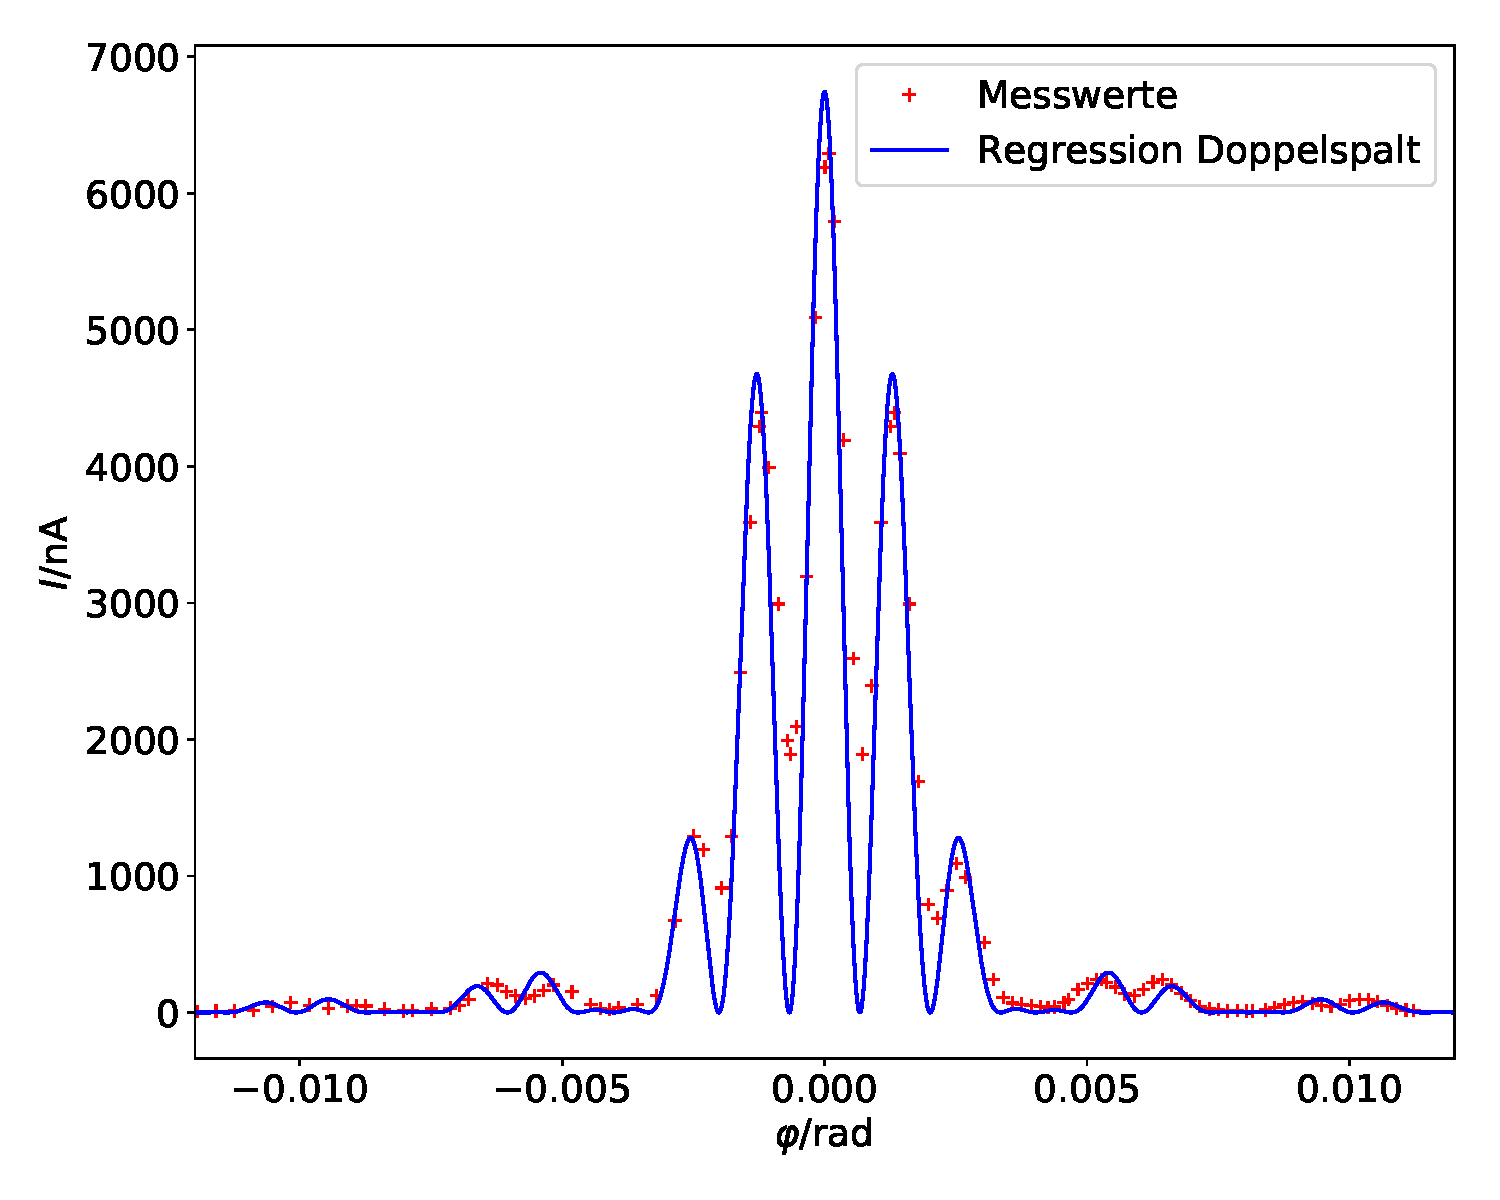
\includegraphics[scale = 0.5]{doppel.pdf}
  \caption{Messwerte und Regression des Doppelspaltes.}
  \label{Abb:3}
\end{figure}

Eine Überlagerung der Regressionen von dem ersten Einzelspalt und dem Doppelspalt in in Abbildung \ref{Abb:4} zu sehen. Um Die Regressionen vergleichen zu können,
muss die Regression des Einzelspaltes mit einem Faktor von $a$ = 2,26 multipliziert werden.

\begin{figure}
  \centering
  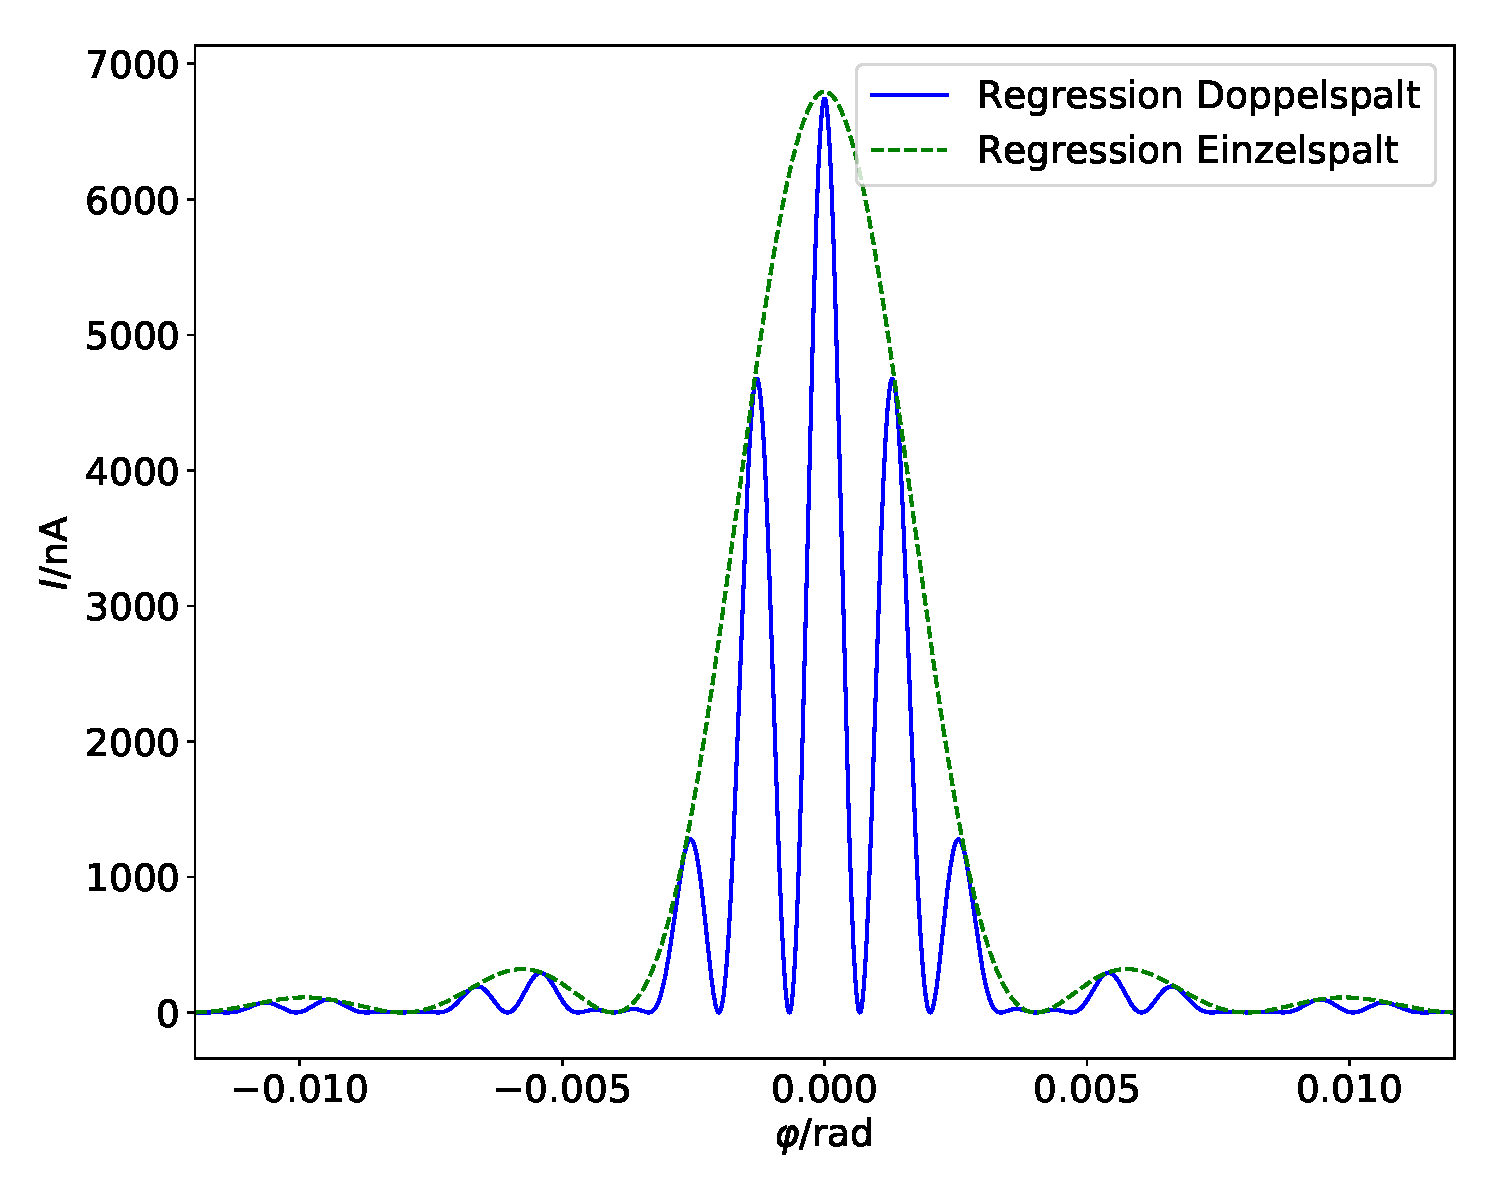
\includegraphics[scale= 0.5]{doppeleinzel.pdf}
  \caption{Überlagerung Einzelspalt und Doppelspalt}
  \label{Abb:4}
\end{figure}

\section{Diskussion}

Die Messwerte werden mit den Literaturwerten mit Hilfe von prozentualen Abweichungen in Tabelle \ref{tab:4} verglichen. Zu erkennen sind geringe Abweichungen bis zu
\SI{6}{\percent}. Zu erklären lassen sich diese Abweichungen durch mögliche Messfehler. Einer davon könnte durch das Umgebungslicht entstanden sein, welches
nie ganz abgeschirmt werden konnte, auch wenn der Dunkelstrom von dem gemessenen Strom schon abgezogen wird.
In Abbildung \ref{Abb:4} sind die Regressionen des ersten Einzelspaltversuches und des Doppelspaltversuches mit einem Proportinalitätsfaktor übereinander gelegt.
Zu erkennen ist, dass die Einzelspaltfunktion die Doppelspaltfunktion perfekt einhüllt.

\begin{table}
  \centering
  \caption{Vergleich Literaturwerte und Messwerte}
  \label{tab:4}
  \begin{tabular}{c | c c | c}
    \toprule
    & Literaturwert & Messwert & prozentuale Abweichung \\
    \midrule
    Einzelspalt 1 & $b$ = \SI{15e-5}{\meter} & $b$ = \SI{14,97(7)e-5}{\meter}  & \SI{0,02}{\percent}  \\
    \midrule
    Einzelspalt 1 & $b$ = \SI{7,5e-5}{\meter} & $b$ = \SI{7,87(8)e-5}{\meter}  &  \SI{4,93}{\percent} \\
    \midrule
    Doppelspalt & $b$ = \SI{15e-5}{\meter} & $b$ = \SI{15,7(6)e-5}{\meter}  &  \SI{4,67}{\percent} \\
    & $s$ = \SI{50e-5}{\meter} & $s$ = \SI{47,2(5)e-5}{\meter} & \SI{5,6}{\percent} \\
    \bottomrule
  \end{tabular}
\end{table}


\nocite{*}
\printbibliography
